\chapter{Related Works}\label{ch:related_works}
In this chapter, we will present the main concepts and projects used and followed during the development of this thesis. 
We will start by presenting rehabilitation approaches and technologies and the importance of the gamification of rehabilitation. 
We will also present the main concepts of the Brain-Computer Interface (BCI) and the most relevant projects that use BCI and more specifically Motor Imagery for rehabilitation and devices control.
Lastly, we will present concepts of usability and game feel that are important for the development of a usable and engaging application.

\begin{figure}[htbp!]
    \centering
    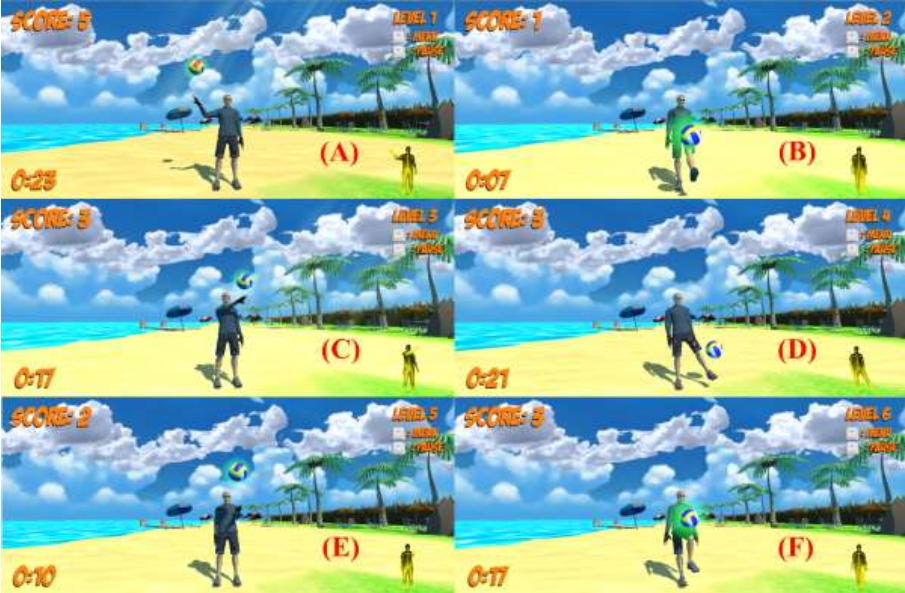
\includegraphics[width=\textwidth]{Figures/Related/ave_exergame}
    \caption{VR Exergame - A BCI-based exergame for rehabilitation. Image from~\cite{trombetta}}\label{fig:exergame}
\end{figure}

\begin{figure}[htbp!]
    \centering
    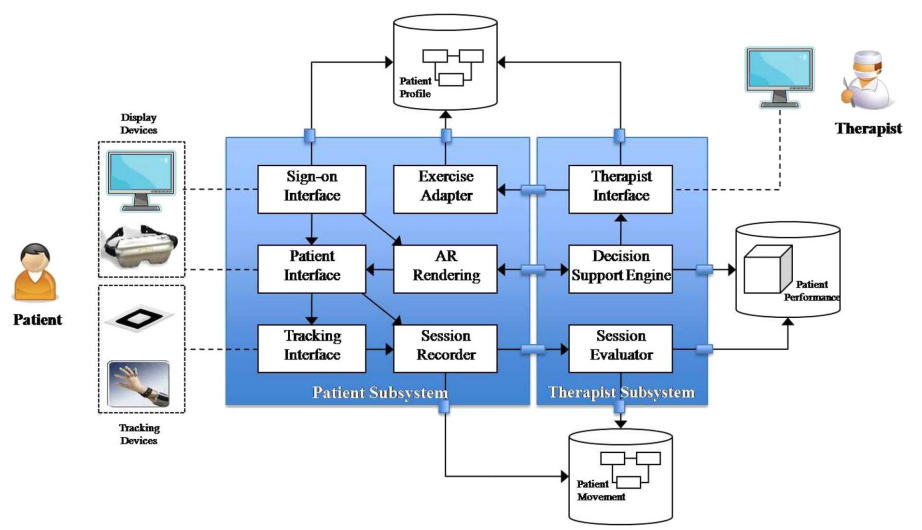
\includegraphics[width=\textwidth]{Figures/Related/ar_app_framework}
    \caption{AR Framework - A framework for the development of AR applications for rehabilitation. Image from~\cite{5567156}}\label{fig:ar_app_framework}
\end{figure}

\section{Rehabilitation Approaches and Technologies}
Rehabilitation is a process that aims to restore the physical, sensory, and mental abilities of individuals who have lost them due to injury, illness, or other health conditions.
There are several approaches to rehabilitation, and the choice of the most appropriate one depends on the patient's condition and the goals to be achieved.
The main approaches to rehabilitation are physical therapy, occupational therapy, and speech therapy.
Physical therapy aims to restore the patient's physical abilities, such as strength, flexibility, and coordination.
Occupational therapy aims to help the patient to perform daily activities, such as eating, dressing, and bathing.
Speech therapy aims to help the patient to improve their communication skills, such as speaking, listening, and understanding language.
There are also other approaches to rehabilitation, such as music therapy, art therapy, and animal-assisted therapy, which can be used to complement the traditional approaches.
Works like~\cite{202306.0333, 5567156, 10.4108/icst.pervasivehealth.2014.255277, trombetta}, aim to further aid the rehabilitation process using AR and VR applications, exergames, and serious games.
For example, in Figure~\ref{fig:exergame}, we can see a VR exergame for upper and lower limbs rehabilitation, while in Figure~\ref{fig:ar_app_framework}, we can see a framework for the development of AR applications for rehabilitation that also aids the medical staff in the monitoring of the progress and performances of the patient, and supports the therapist in deciding the most appropriate exercises for the patient.
In~\cite{BOUKHENNOUFA2022103197}, we can also find a review of state of the art solutions that involve werable sensors and machine learning techniques.
In the last decades, the use of Brain Computer Interfaces (BCI) has been gaining popularity in the field of rehabilitation, as they allow the control of devices and applications using only the brain signals.
The work from Bai et al.~\cite{bai_immediate_2020} analyzes short and long term effects of BCI-based rehabilitation systems and concludes that these interfaces are safe for patients with strokes and effective at improving upper extremity motor function.
The review~\cite{alfieri_gamification_2022} shows that gamification provides improved rehabilitation results compared to conventional therapy or home-based exercises, and can improve the motivation and engagement of patients in rehabilitation exercises.

\begin{figure}[htbp!]
    \centering
    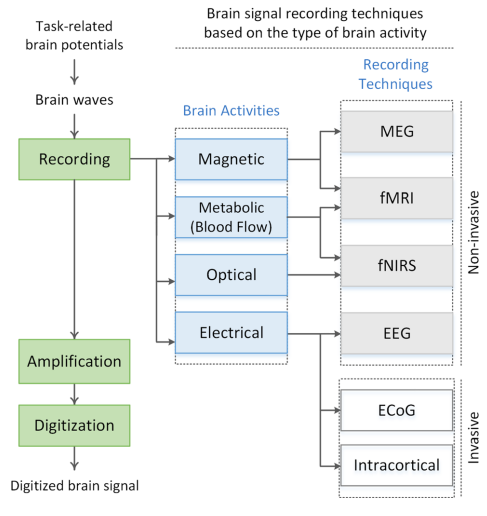
\includegraphics[width=0.5\textwidth]{Figures/Related/brain_signal_recording_techniques}
    \caption{Brain Signal Recording Techniques - A list of the most common brain signal recording techniques. Image from~\cite{altaheri2023deep}}\label{fig:brain_signal_recording_techniques}
\end{figure}
\section{Brain-Computer Interfaces (BCI)}
Brain Computer Interfaces are links between the brain and electronic devices, such as computers, smartphones, and robots.
These interfaces allow the control of devices and applications using only the brain signals.
In~\cite{robinson2021emerging}, the authors review the current state of the art for BCI technologies used to control robots and for motor rehabilitation.
In their work, they present the main types of BCI, such as invasive, and non-invasive, and the most common non-invasive signal acquisition methods, such as Electroencephalography (EEG)~\cite{niedermeyer2005electroencephalography} and Magnetoencephalography (MEG)~\cite{singh2014magnetoencephalography}, a comprehensive list of the most common brain signal recording techniques can be found in Figure~\ref{fig:brain_signal_recording_techniques}.
In~\cite{altaheri_deep_2023}, Altaheri et al.\ present the EEG Motor Imagery as one of the ``most common BCI paradigms that have been used extensively in smart healthcare applications such as poststroke rehabilitation and mobile assistive robots''.
In this work, the authors also review existing applications, like~\cite{tang2020motor} that presents an EEG MI system used to control a wheelchair, publicly available datasets for EEG Motor Imagery, such as the ones from the BCI Competition IV~\cite{tangermann2012review}, the one from the Yi, Weibo et al.~\cite{yi2014evaluation} and the ones provided by PhysioNet~\cite{goldberger2000physiobank, schalk2004bci2000}, and present the most common deep learning algorithms used for EEG Motor Imagery classification, such as Convolutional Neural Networks (CNN)~\cite{lawhern2018eegnet}, Long Short-Term Memory (LSTM) and Transformer Based solutions~\cite{sharma_deep_2023}.
In the filed of controlling devices using EEG, also other works were identified, such as~\cite{10471624}, where the author present a werable device that is used to control a wheelchair, and~\cite{10453986}, where the author presents a system that uses electromyography (EMG)~\cite{mills2005basics} to control artificial limbs.
We also found relevant for this project, the work~\cite{ahn2013gamma} where the authors explore the effect of gamma band in MI to improve BCI performances.
Also, we will consider, as in~\cite{mammone2023few}, the possibility of applying few-shot learning to tailor the EEG MI classification networks to the user's brain signals.
Lastly, altrough not directly related to the development of the EEG MI system for this thesis, we found relevant the work from~\cite{10123901, lee2022individual}, where the authors explore the possibility of detecting individual finger movements and hand gestures using ultra high density EEG, and the work from~\cite{penfield1950cerebral, jasper1958ten}, where the authors present the motor homunculus and the International 10-20 System (Figure~\ref{fig:international_10_20_system}) for EEG electrode placement.
Also, Figure~\ref{fig:brain_lobes} is provided as reference to understand wich area of the brain is recorded by the EEG electrodes.

\begin{figure}[htbp!]
    \centering
    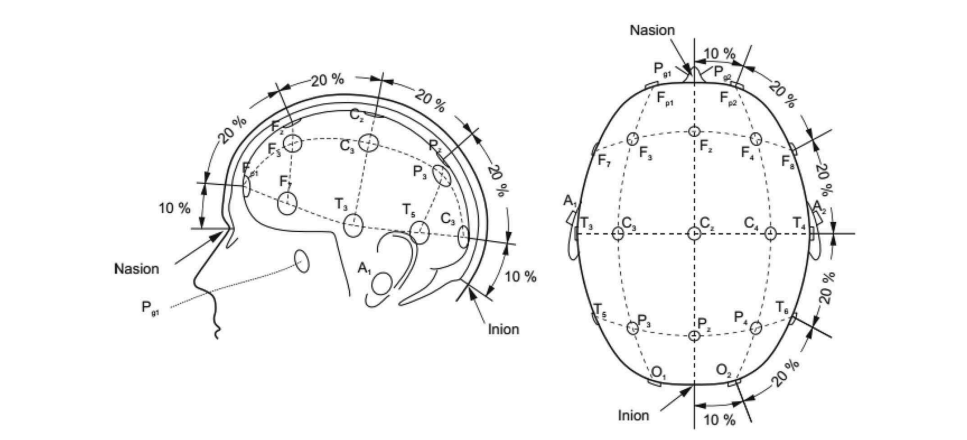
\includegraphics[width=0.45\textwidth]{Figures/Related/international_10_20_system}
    \caption{International 10-20 System. Image from~\cite{luis2012brain}}\label{fig:international_10_20_system}
\end{figure}
\begin{figure}[htbp!]
    \centering
    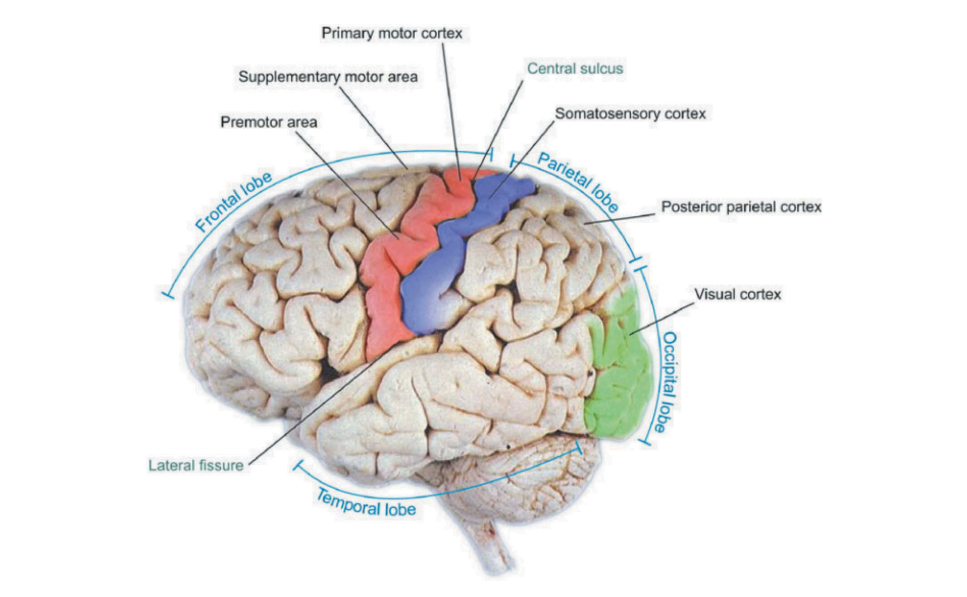
\includegraphics[width=0.45\textwidth]{Figures/Related/brain_lobes}
    \caption{Brain Lobes. Image from~\cite{Harrison2015}}\label{fig:brain_lobes}
\end{figure}

\section{Usability and Game Feel}
Usability is a key factor in the development of applications, as it can influence the user's experience and satisfaction.
Is commonly defined as the ease of use and learnability of an application, but cannot be measured directly, as it depends on the user's perception and experience.
In~\cite{swink2008game}, the author presents the main concepts of game feel in video games, such as responsiveness, smoothness, and consistency, and how they can be used to improve the user experience and the game flow.
In~\cite{perez2018virtual}, the author provides a list of characteristics that impact the feel of a realistic virtual reality environment, along with measures for assessing these characteristics.
Immersion, interaction, sensorimotor contingencies,such spatiotemporal correlation, and the impression of presence are examples of these attributes.
The article also explains how these characteristics impact the user experience. 
The thesis from Nguyen~\cite{nguyen2012human}, shows that there is a weak correlation between Human Computer Interaction and Game Design, and suggests the use of heuristics and character automation to improve the overall user experience.
In~\cite{doi:10.1080/10447318.2019.1612213}, the authors present a review of the main videogames developed for consumer grade EEG devices.
The authors mention that many works only had simplified controls and used attention and meditation signals, also, only few research works were focused on the usability and qualitative aspects of the user interaction with the games.

\section{Main Differences}
Using these works and documents as a reference, we can see that there is a gap in the literature regarding the development of a BCI-based application that is both usable and engaging.
Most of the works focus on the technical aspects of the BCI, such as signal acquisition and processing, and the development of the rehabilitation exercises, but do not focus on the usability and user experience of the application.
In this thesis, we aim to fill this gap by developing a BCI-based application that is both usable and engaging, and by evaluating the user experience of the application using a mixed-methods approach.
Our project will use the BCI Motor Imagery paradigm to control an application, we will not specifically focus on rehabilitation exercises, but we will develop simple videogames aiming to provide a good level of usability and a fun and immersive experience to the final user.
The games will be controlled by the immagination of movements of hands and feet, and the user will be able to play them using only their brain signals.
Lastly, to test the games and the networks developed during this thesis, we will develop a tool to generate artificial data, that will be fundamental in the early testing stages.
